\documentclass[12pt,a4paper]{article}
\usepackage[utf8]{inputenc}
\usepackage[english]{babel}
%\usepackage{minted}
\usepackage{listings}
\usepackage{xcolor}
\usepackage{graphicx}

%For syntax highlighting
\definecolor{codegreen}{rgb}{0,0.6,0}
\definecolor{codegray}{rgb}{0.5,0.5,0.5}
\definecolor{codepurple}{rgb}{0.58,0,0.82}
\definecolor{backcolour}{rgb}{1,1,1}

%%Sets different parameters
\lstdefinestyle{mystyle}{
	backgroundcolor=\color{backcolour},   
    commentstyle=\color{codegreen},
    keywordstyle=\color{magenta},
    numberstyle=\tiny\color{codegray},
    stringstyle=\color{codepurple},
    basicstyle=\ttfamily\footnotesize,
    breakatwhitespace=false,         
    breaklines=true,                 
    captionpos=b,                    
    keepspaces=true,                 
    numbers=left,                    
    numbersep=5pt,                  
    showspaces=false,                
    showstringspaces=false,
    showtabs=false,                  
    tabsize=4
}
\lstset{style=mystyle}

\title{\bf Case Conversion}
\author{\vspace{-10ex}}
\date{\vspace{-10ex}}
\begin{document}
\maketitle

\begin{minipage}{0.45\textwidth}
        \begin{tabular}{l l}
            \textbf{Expt No:}&8\\
            \textbf{Date :}&16/10/2020
        \end{tabular}
\end{minipage}%
\begin{minipage}{0.45\textwidth}
        \begin{tabular}{l l}
             \textbf{Name:}& Shivanirudh S G  \\
             \textbf{Reg No:} & 185001146 
        \end{tabular}
\end{minipage}
\vspace{1cm}
\hrule

\begin{flushleft}
\subsection*{\textbf{Aim:}} 
To convert case of characters from keyboard on the move in 8086.

\vspace{1cm}
\hrule

\subsubsection*{\textbf{Algorithm:}}
\begin{itemize}
    \item Move the data segment to the AX register and then move it to the DS register.
    \item Move value of count to CX register.
    \item Move value 1 to AH register, under label L1.
    \item Request interrupt 21H to enable keyboard input stored AL register. 
    \item Compare AL with hex value 60 using CMP AL, 60H. 
    \item Jump to label UPPER if AL is greater than 60.
    \item Add hex value 20H to AL using ADD AL, 20H.
    \item Jump to label DONE.
    \item Subtract hex value 20H from AL using SUB AL, 20H under label UPPER.
    \item Move value 2 to AH register, under label DONE.
    \item Move contents to AL to DL register to display it.
    \item Request interrupt 21H to enable output at standard output.
    \item Loop back to label L1.
\end{itemize}

\newpage
\subsubsection*{\textbf{Program:}}

\begin{table}[htb]
\centering
\resizebox{\columnwidth}{!}{
\begin{tabular}{|l|l|} 
\hline
\textbf{Program}                                                 & \textbf{Comments}                             \\ 
\hline
\hline
assume cs:code, ds:data                                          & Declare code and data segments                \\
\hline
data segment                                                     & Start of data segment                         \\
\hline
count equ 10H                                                    & Define variable count with value 10H          \\
\hline
data ends                                                        & End of data segment                           \\
\hline
code segment                                                     & Start of code segment                         \\
\hline
start:~mov ax, data                                              & Move data to AX register                      \\
\hline
mov ds, ax                                                       & Move contents of AX register to DS register   \\
\hline
mov cx, count                                                    & Move value of count to CX register            \\
\hline
l1:~mov ah, 1                                                    & Move value 1 o AH register                    \\
\hline
int 21h                                                          & Accept keyboard input                         \\
\hline
cmp al, 60H                                                      & Compare value in AL register with hex value 60\\
\hline
jnc upper                                                        & Jump to upper if AL > 60                      \\
\hline
add al, 20H                                                      & AL = AL + 20                                  \\
\hline
jmp done                                                         & Jump to done                                  \\
\hline
upper:~sub al, 20H                                               & AL = AL - 20                                  \\
\hline
done:~mov ah, 2                                                  & Move value 2 to AH register                   \\
\hline
mov dl, al                                                       & Move value in AL register to DL register      \\
\hline
int 21h                                                          & Display value in standard output              \\
\hline
loop l1                                                          & Loop back from L1                             \\
\hline
mov ah, 4ch                                                & To request interrupt                          \\
\hline
int 21h                                                          & Request interrupt routine                     \\ 
\hline
code ends                                                        & End of code segment                           \\
\hline
end start                                                        &                                               \\
\hline
\end{tabular}
}
\end{table}

\newpage
\subsection*{\textbf{Unassembled code:}}
\begin{figure}[h]
    \centering
    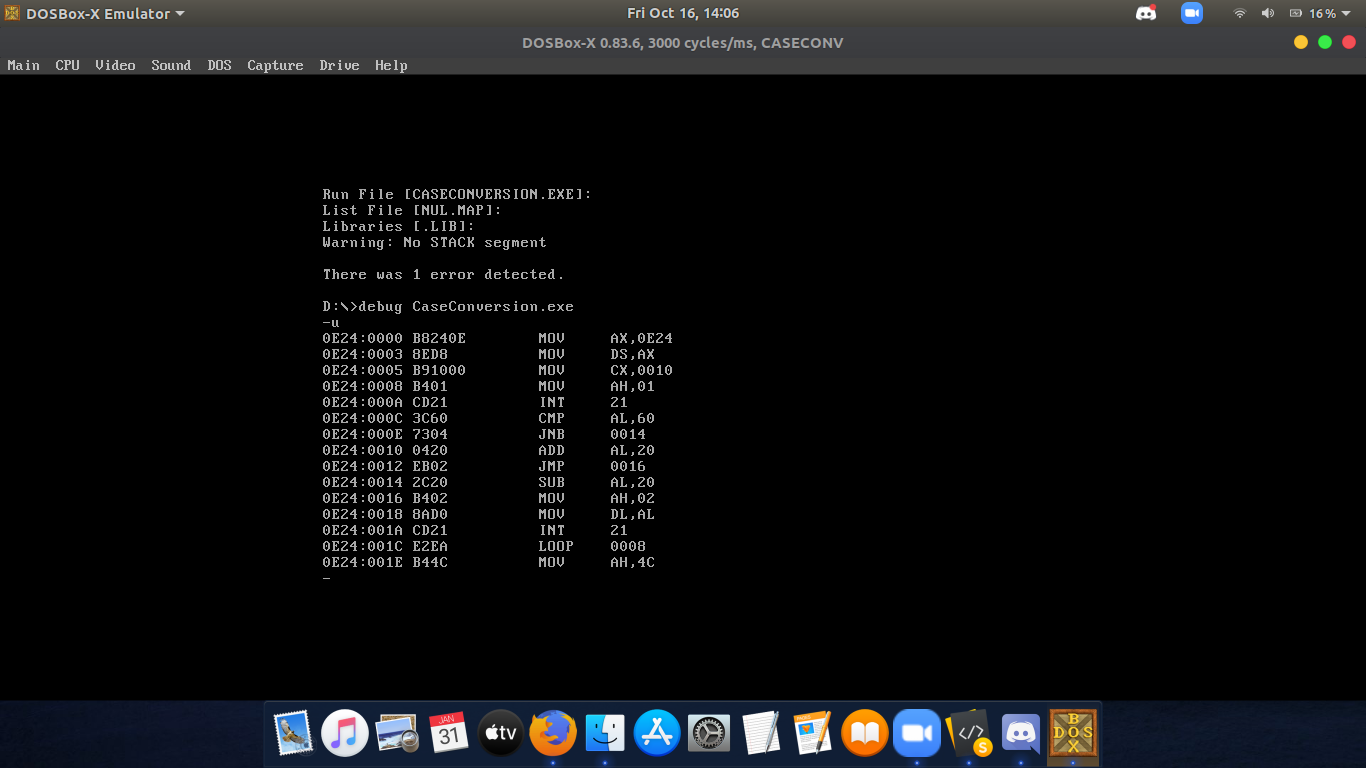
\includegraphics[trim = 100mm 60mm 200mm 110mm, clip, width = \textwidth]{Pics/CaseUS.png}
\end{figure}
\subsubsection*{\textbf{Input and Output:}}
\begin{figure}[h]
    \centering
    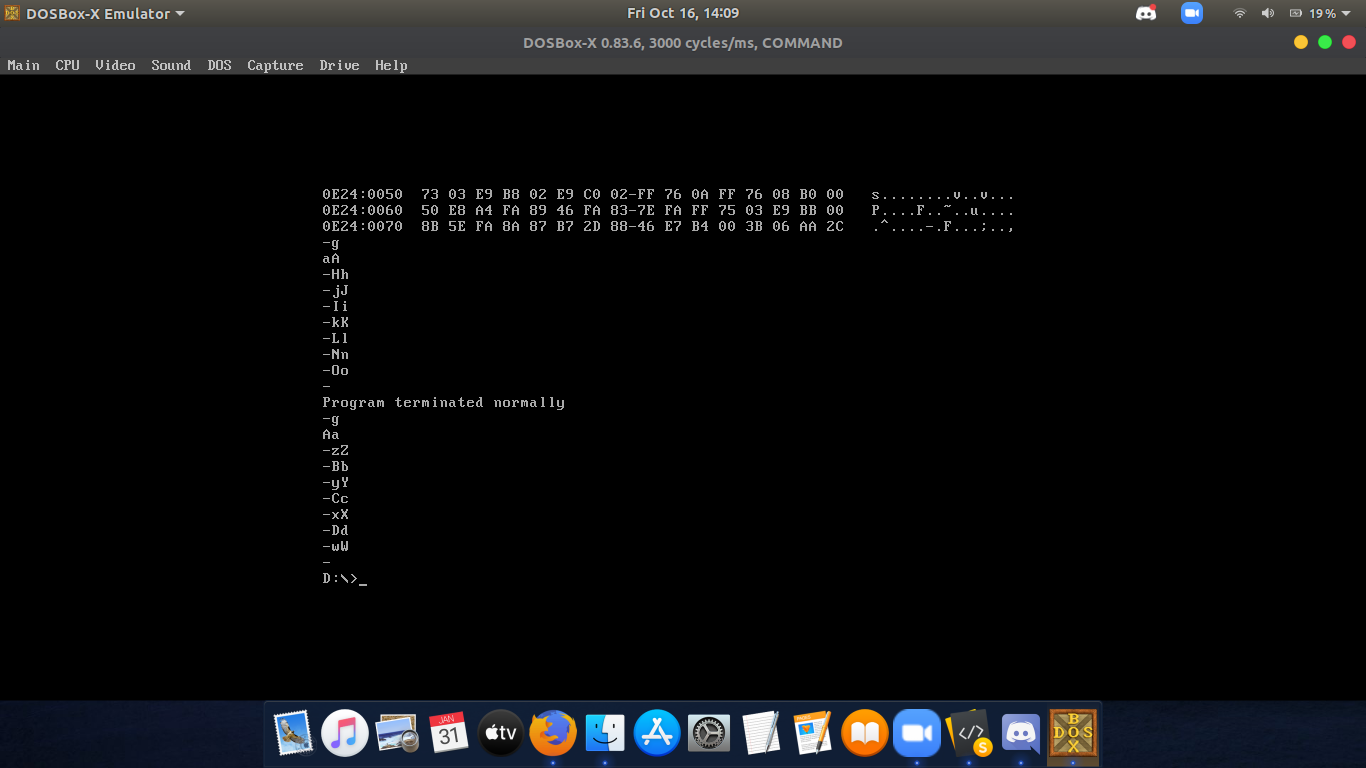
\includegraphics[trim = 100mm 60mm 100mm 145mm, clip, width = \textwidth]{Pics/CaseIO.png}
    \caption{ \textbf{Input:} A, z, B, y, C, x, D, w  ; \newline \hspace{1cm}
              \textbf{Output:} a, Z, b, Y, c, X, d, W}
\end{figure}
\hrule
\subsection*{\textbf{Result:}}
The 8086 programs were written to perform matrix operations, and the results observed.
\end{flushleft}
\end{document}